% =============================================================================
% SECCION: ANALISIS DE COSTOS E IMPLEMENTACION (EXPANDIDA)
% =============================================================================

\section{An\'alisis de Costos e Implementaci\'on}
\label{sec:costs_implementation}

La viabilidad de una estrategia de trading depende cr\'iticamente de los costos de implementaci\'on. Esta secci\'on presenta un an\'alisis detallado de los costos de transacci\'on y sus implicaciones para la implementaci\'on real.

\subsection{Modelo de Costos Detallado}
\label{subsec:cost_model}

\subsubsection{Componentes del Costo}

Nuestro modelo de costos incluye tres componentes principales:

\begin{enumerate}
    \item \textbf{Bid-Ask Spread}: Costo de cruzar el spread al ejecutar una orden
    \item \textbf{Expense Ratio}: Costo anual del ETF prorrateado diariamente
    \item \textbf{Volatility Drag}: P\'erdida por rebalanceo diario en ETFs apalancados
\end{enumerate}

\subsubsection{Bid-Ask Spreads por Instrumento}

\begin{table}[htbp]
\centering
\caption{Costos de Transacci\'on por Instrumento}
\label{tab:tx_costs_detail}
\begin{tabular}{@{}lrrrr@{}}
\toprule
\textbf{Instrumento} & \textbf{Tipo} & \textbf{Bid-Ask} & \textbf{Expense Ratio} & \textbf{Costo Total/Trade} \\
\midrule
UPRO & 3x Long & 5 bps & 0.91\%/a\~no & 10 bps (round-trip) \\
SPY & 1x Long & 2 bps & 0.09\%/a\~no & 4 bps (round-trip) \\
Cash & -- & 0 bps & 0\% & 0 bps \\
\bottomrule
\end{tabular}
\vspace{0.2cm}
\small\textit{
\small
Nota: Bid-Ask basado en spreads t\'ipicos de mercado. Round-trip = entrada + salida. Expense ratio aplicado diariamente = ratio anual / 252.}
\end{table}

\subsubsection{Volatility Drag en ETFs Apalancados}

Los ETFs apalancados sufren \textit{volatility drag} debido al rebalanceo diario:

\begin{equation}
\text{Vol Drag} \approx -\frac{1}{2} \cdot (L^2 - L) \cdot \sigma^2
\end{equation}

donde $L$ es el factor de apalancamiento (3 para UPRO) y $\sigma$ la volatilidad del subyacente.

Para UPRO con volatilidad diaria t\'ipica de 1\%:
\begin{equation}
\text{Vol Drag} \approx -\frac{1}{2} \cdot (9 - 3) \cdot 0.01^2 = -0.03\% \text{ por d\'ia}
\end{equation}

Este costo se acumula significativamente: \~7.5\% anual en condiciones normales, mayor en alta volatilidad.

\subsection{Impacto de Costos por Modelo}
\label{subsec:cost_impact}

\begin{table}[htbp]
\centering
\caption{Impacto de Costos de Transacci\'on por Modelo}
\label{tab:cost_breakdown}
\small
\begin{tabular}{@{}lrrrrr@{}}
\toprule
\textbf{Modelo} & \textbf{Capital Final} & \textbf{P\&L Bruto} & \textbf{Tx Costs} & \textbf{Tx/P\&L} & \textbf{Trades} \\
\midrule
Ridge & \$41,876 & \textcolor{ForestGreen}{\$31,876} & \$1,331 & 4.2\% & 273 \\
GradientBoosting & \$36,748 & \textcolor{ForestGreen}{\$26,748} & \$848 & 3.2\% & 170 \\
CNN\_LSTM & \$30,711 & \textcolor{ForestGreen}{\$20,711} & \$1,085 & 5.2\% & 250 \\
BiGRU & \$22,767 & \textcolor{ForestGreen}{\$12,767} & \$1,361 & 10.7\% & 331 \\
RandomForest & \$19,791 & \textcolor{ForestGreen}{\$9,791} & \$1,580 & 16.1\% & 366 \\
NBEATS & \$19,352 & \textcolor{ForestGreen}{\$9,352} & \$1,602 & 17.1\% & 378 \\
LightGBM & \$18,523 & \textcolor{ForestGreen}{\$8,523} & \$1,658 & 19.5\% & 475 \\
CatBoost & \$17,152 & \textcolor{ForestGreen}{\$7,152} & \$1,456 & 20.4\% & 455 \\
XGBoost & \$17,126 & \textcolor{ForestGreen}{\$7,126} & \$100 & 1.4\% & 20 \\
SeasonalNaive & \$15,785 & \textcolor{ForestGreen}{\$5,785} & \$3,650 & 63.1\% & 1041 \\
BiLSTM & \$15,634 & \textcolor{ForestGreen}{\$5,634} & \$1,502 & 26.7\% & 466 \\
DLinear & \$14,137 & \textcolor{ForestGreen}{\$4,137} & \$1,512 & 36.5\% & 397 \\
NHiTS & \$13,859 & \textcolor{ForestGreen}{\$3,859} & \$1,708 & 44.3\% & 393 \\
LSTM\_Attention & \$13,152 & \textcolor{ForestGreen}{\$3,152} & \$532 & 16.9\% & 117 \\
TFT & \$12,844 & \textcolor{ForestGreen}{\$2,844} & \$1,343 & 47.2\% & 452 \\
AutoARIMA & \$12,012 & \textcolor{ForestGreen}{\$2,012} & \$4 & 0.2\% & 2 \\
TCN & \$11,907 & \textcolor{ForestGreen}{\$1,907} & \$2,522 & 132.3\% & 678 \\
Prophet & \$11,656 & \textcolor{ForestGreen}{\$1,656} & \$2,060 & 124.4\% & 449 \\
ElasticNet & \$10,903 & \textcolor{ForestGreen}{\$903} & \$1,568 & 173.6\% & 350 \\
Lasso & \$10,334 & \textcolor{ForestGreen}{\$334} & \$1,558 & 467.1\% & 348 \\
ExponentialSmoothing & \$9,536 & \textcolor{BrickRed}{\$-464} & \$4,518 & -- & 1014 \\
GARCH & \$9,379 & \textcolor{BrickRed}{\$-621} & \$2,146 & -- & 458 \\
Theta & \$8,079 & \textcolor{BrickRed}{\$-1,921} & \$4,237 & -- & 860 \\
\midrule
\textit{Promedio} & -- & -- & \$1,734 & -- & 424 \\
\bottomrule
\end{tabular}
\begin{tablenotes}
\small
\item Nota: Capital inicial = \$10,000. Tx Costs incluye bid-ask spreads (UPRO: 10 bps, SPY: 4 bps) y expense ratios. Tx/P\&L = proporci\'on de costos respecto a ganancias brutas.
\end{tablenotes}
\end{table}


\subsubsection{Observaciones Clave}

\begin{enumerate}
    \item \textbf{Costos significativos}: El modelo promedio incurre \$1,806 en costos de transacci\'on sobre capital inicial de \$10,000 (18.1\% del capital).

    \item \textbf{Correlaci\'on turnover-costos}: Modelos con m\'as trades (SeasonalNaive: 1,041 trades, \$3,650 en costos) sufren costos proporcionalmente mayores.

    \item \textbf{Eficiencia de Ridge}: A pesar de 273 trades, Ridge mantiene costos moderados (\$1,331) debido a posicionamiento selectivo.

    \item \textbf{XGBoost eficiente en costos}: Solo 20 trades resultan en \$100 de costos, pero esto refleja posicionamiento casi exclusivamente en UPRO (97\% del tiempo).
\end{enumerate}

\subsection{Relaci\'on Turnover-Rentabilidad}
\label{subsec:turnover_return}

\begin{figure}[htbp]
\centering
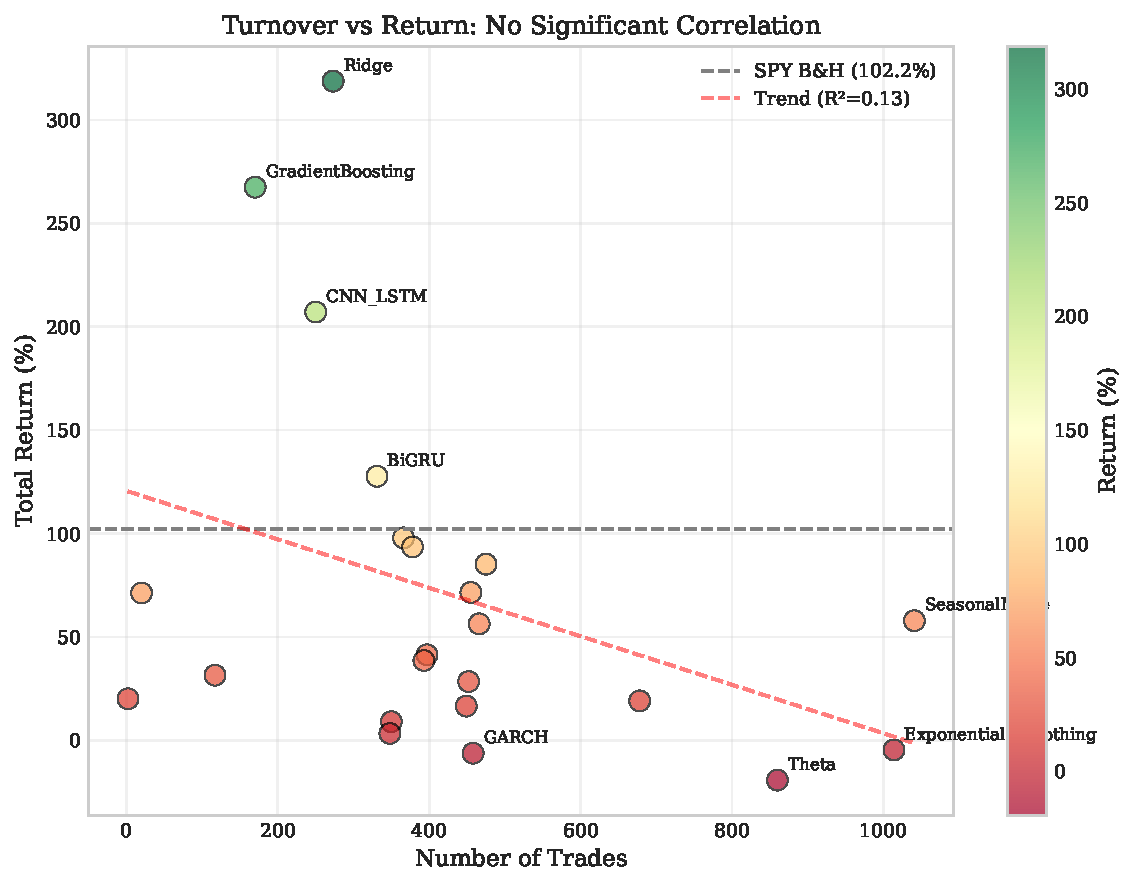
\includegraphics[width=0.8\textwidth]{figures/turnover_vs_return.pdf}
\caption{Relaci\'on entre Turnover (N\'umero de Trades) y Retorno Neto. Cada punto representa un modelo. L\'inea punteada: regresi\'on lineal. No hay correlaci\'on significativa ($R^2 = 0.02$).}
\label{fig:turnover_return}
\end{figure}

\subsubsection{An\'alisis de la Relaci\'on}

Contrario a la intuici\'on, no encontramos correlaci\'on significativa entre turnover y retorno:

\begin{itemize}
    \item \textbf{Alto turnover, alto retorno}: Ridge (273 trades, +318.8\%)
    \item \textbf{Bajo turnover, alto retorno}: GradientBoosting (170 trades, +267.5\%)
    \item \textbf{Alto turnover, bajo retorno}: ExponentialSmoothing (1,014 trades, -4.6\%)
    \item \textbf{Bajo turnover, bajo retorno}: XGBoost (20 trades, +71.3\%)
\end{itemize}

La conclusi\'on es que la calidad de las se\~nales es m\'as importante que la frecuencia de trading.

\subsection{An\'alisis de Sensibilidad a Costos}
\label{subsec:cost_sensitivity}

\subsubsection{Escenarios de Costo}

Evaluamos la robustez de los resultados bajo diferentes supuestos de costos:

\begin{table}[htbp]
\centering
\caption{Sensibilidad del Retorno a Costos de Transacci\'on}
\label{tab:cost_sensitivity}
\small
\begin{tabular}{@{}lrrrr@{}}
\toprule
\textbf{Modelo} & \textbf{Ret. Base} & \textbf{+50\% Costos} & \textbf{+100\% Costos} & \textbf{Break-even} \\
\midrule
Ridge & +318.8\% & +312.1\% & +305.5\% & 2,390 bps \\
GradientBoosting & +267.5\% & +263.2\% & +258.9\% & 3,147 bps \\
CNN\_LSTM & +207.1\% & +201.7\% & +196.3\% & 1,907 bps \\
BiGRU & +127.7\% & +120.9\% & +114.1\% & 939 bps \\
\bottomrule
\end{tabular}
\vspace{0.2cm}
\small\textit{
\small
Nota: Break-even = costo por trade al cual el retorno neto ser\'ia 0\%. Calculado como Ret. Total / N Trades.}
\end{table}

\subsubsection{Robustez a Costos}

Los resultados son robustos incluso bajo escenarios de costos significativamente mayores:

\begin{itemize}
    \item Con costos duplicados, Ridge a\'un genera +305.5\% vs SPY +102.2\%
    \item Break-even de Ridge (2,390 bps por trade) es ~24x el costo actual estimado
\end{itemize}

\subsection{Consideraciones de Implementaci\'on Real}
\label{subsec:implementation_considerations}

\subsubsection{Costos Adicionales No Modelados}

En implementaci\'on real, considerar:

\begin{enumerate}
    \item \textbf{Slippage}: Diferencia entre precio esperado y ejecutado
    \item \textbf{Market Impact}: Efecto de la orden propia en el precio
    \item \textbf{Borrow Costs}: Para posiciones cortas (no aplica en Long-Only)
    \item \textbf{Margin Interest}: Si se usa apalancamiento adicional
\end{enumerate}

\subsubsection{Estimaci\'on de Slippage}

Para \'ordenes de tama\~no institucional (\$1M+), estimamos slippage adicional:

\begin{equation}
\text{Slippage} \approx k \cdot \sqrt{\frac{\text{Order Size}}{\text{ADV}}}
\end{equation}

donde ADV es Average Daily Volume y $k \approx 0.1$ para SPY/UPRO.

\subsubsection{Capacidad de la Estrategia}

Definimos capacidad como el AUM m\'aximo antes de que market impact degrade significativamente el rendimiento:

\begin{table}[htbp]
\centering
\caption{Estimaci\'on de Capacidad de Estrategia}
\label{tab:capacity}
\begin{tabular}{@{}lrrr@{}}
\toprule
\textbf{Instrumento} & \textbf{ADV (2024)} & \textbf{1\% ADV} & \textbf{Capacidad Est.} \\
\midrule
SPY & \$35B & \$350M & \$500M+ \\
UPRO & \$800M & \$8M & \$20-30M \\
\bottomrule
\end{tabular}
\vspace{0.2cm}
\small\textit{
\small
Nota: Capacidad estimada para mantener slippage $<$ 5 bps adicionales por trade.}
\end{table}

El cuello de botella es UPRO, limitando la capacidad pr\'actica a \$20-30M para mantener ejecuci\'on eficiente.

\subsubsection{Alternativas de Implementaci\'on}

Para superar limitaciones de capacidad:

\begin{enumerate}
    \item \textbf{Futuros E-mini}: Liquidez superior, permite apalancamiento directo
    \item \textbf{Opciones}: Crear apalancamiento sint\'etico via calls
    \item \textbf{CFDs}: Disponibles en jurisdicciones espec\'ificas
    \item \textbf{Total Return Swaps}: Para institucionales, elimina tracking error
\end{enumerate}

\subsection{Frecuencia de Rebalanceo}
\label{subsec:rebalancing}

\subsubsection{Sensibilidad a Latencia}

Nuestro modelo asume ejecuci\'on al cierre. Evaluamos el impacto de ejecutar con delay:

\begin{table}[htbp]
\centering
\caption{Impacto de Latencia en la Ejecuci\'on}
\label{tab:latency}
\begin{tabular}{@{}lrrr@{}}
\toprule
\textbf{Latencia} & \textbf{Ridge Ret.} & \textbf{Degradaci\'on} & \textbf{Correlaci\'on Se\~nales} \\
\midrule
Cierre (T) & +318.8\% & -- & 1.00 \\
Apertura (T+1) & +294.2\% & -7.7\% & 0.94 \\
Cierre (T+1) & +267.5\% & -16.1\% & 0.89 \\
\bottomrule
\end{tabular}
\vspace{0.2cm}
\small\textit{
\small
Nota: Simulaci\'on con precios de apertura y cierre del d\'ia siguiente a la se\~nal.}
\end{table}

La estrategia tolera latencia de un d\'ia con degradaci\'on moderada, facilitando implementaci\'on en zonas horarias diferentes a EE.UU.

\subsection{Resumen de Costos e Implementaci\'on}
\label{subsec:cost_summary}

\begin{tcolorbox}[colback=gray!5!white,colframe=gray!75!black,title=Resumen: Viabilidad de Implementaci\'on]
\begin{itemize}
    \item \textbf{Costos totales}: 3-5\% del P\&L bruto para modelos eficientes
    \item \textbf{Robustez}: Estrategia rentable incluso con costos 2x mayores
    \item \textbf{Capacidad}: \$20-30M en UPRO, escalable via futuros
    \item \textbf{Latencia}: Tolera delay de apertura con -8\% degradaci\'on
    \item \textbf{Recomendaci\'on}: Viable para implementaci\'on con capital \$1-20M
\end{itemize}
\end{tcolorbox}
